\subsection{Linux versioning scheme and development process}

\begin{frame}
  \frametitle{Until 2.6 (1)}
  \begin{itemize}
  \item One stable major branch every 2 or 3 years
    \begin{itemize}
    \item Identified by an even middle number
    \item Examples: \code{1.0.x, 2.0.x, 2.2.x, 2.4.x}
    \end{itemize}
  \item One development branch to integrate new functionalities and
    major changes
    \begin{itemize}
    \item Identified by an odd middle number
    \item Examples: \code{2.1.x, 2.3.x, 2.5.x}
    \item After some time, a development version becomes the new base
      version for the stable branch
    \end{itemize}
  \item Minor releases once in while: \code{2.2.23, 2.5.12}, etc.
  \end{itemize}
\end{frame}

\begin{frame}
  \frametitle{Until 2.6 (2)}
  \begin{center}
    \includegraphics[width=\textwidth]{slides/sysdev-linux-intro-versioning/old-development-process.pdf}
  \end{center} \end{frame}

\begin{frame}
  \frametitle{Changes since Linux 2.6}
  \begin{itemize}
  \item Since \code{2.6.0}, kernel developers have been able to
    introduce lots of new features one by one on a steady pace,
    without having to make disruptive changes to existing subsystems.
  \item Since then, there has been no need to create a new development branch
    massively breaking compatibility with the stable branch.
  \item Thanks to this, {\bf more features are released to users at a
      faster pace}.
  \end{itemize}
\end{frame}

\begin{frame}
  \frametitle{3.x stable branch}
  \begin{itemize}
  \item From 2003 to 2011, the official kernel versions were named \code{2.6.x}.
  \item Linux \code{3.0} was released in July 2011
  \item This is only a change to the numbering scheme
    \begin{itemize}
    \item Official kernel versions are now named \code{3.x}
      (\code{3.0, 3.1, 3.2}, etc.)
    \item Stabilized versions are named \code{3.x.y}
      (\code{3.0.2, 3.4.3}, etc.)
    \item It effectively only removes a digit compared to the previous
      numbering scheme
    \end{itemize}
  \end{itemize}
\end{frame}

\begin{frame}
  \frametitle{New development model}
  Using merge and bug fixing windows
  \begin{center}
    \includegraphics[width=\textwidth]{slides/sysdev-linux-intro-versioning/new-development-process.pdf}
  \end{center}
\end{frame}

\begin{frame}
  \frametitle{New development model - Details}
  \begin{itemize}
  \item After the release of a \code{3.x} version (for example),
    a two-weeks merge window opens, during which major additions are merged.
  \item The merge window is closed by the release of test version
    \code{3.(x+1)-rc1}
  \item The bug fixing period opens, for 6 to 10 weeks.
  \item At regular intervals during the bug fixing period,
    \code{3.(x+1)-rcY} test versions are released.
  \item When considered sufficiently stable, kernel \code{3.(x+1)}
    is released, and the process starts again.
  \end{itemize}
\end{frame}

\begin{frame}
  \frametitle{More stability for the kernel source tree}
  \begin{columns}
    \column{0.7\textwidth}
    \begin{itemize}
    \item Issue: bug and security fixes only released for most recent
      stable kernel versions.
    \item Some people need to have a recent kernel, but with long term
      support for security updates.
    \item You could get long term support from a commercial embedded
      Linux provider.
    \item You could reuse sources for the kernel used in Ubuntu Long
      Term Support releases (5 years of free security updates).
    \item The \url{http://kernel.org} front page shows which 
      versions will be supported for some time (up to 2 or 3 years),
      and which ones won't be supported any more ("EOL: End Of Life")
    \end{itemize}
    \column{0.3\textwidth}
    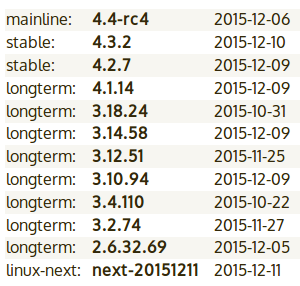
\includegraphics[width=\textwidth]{slides/sysdev-linux-intro-versioning/longterm-versions.png}
  \end{columns}
\end{frame}

\begin{frame}[fragile]
  \frametitle{What's new in each Linux release?}
  \begin{itemize}
  \item The official list of changes for each Linux release is just a
    huge list of individual patches!
\Tiny
    \begin{verbatim}
commit aa6e52a35d388e730f4df0ec2ec48294590cc459
Author: Thomas Petazzoni <thomas.petazzoni@free-electrons.com>
Date:   Wed Jul 13 11:29:17 2011 +0200

    at91: at91-ohci: support overcurrent notification

    Several USB power switches (AIC1526 or MIC2026) have a digital output
    that is used to notify that an overcurrent situation is taking
    place. This digital outputs are typically connected to GPIO inputs of
    the processor and can be used to be notified of those overcurrent
    situations.

    Therefore, we add a new overcurrent_pin[] array in the at91_usbh_data
    structure so that boards can tell the AT91 OHCI driver which pins are
    used for the overcurrent notification, and an overcurrent_supported
    boolean to tell the driver whether overcurrent is supported or not.

    The code has been largely borrowed from ohci-da8xx.c and
    ohci-s3c2410.c.

    Signed-off-by: Thomas Petazzoni <thomas.petazzoni@free-electrons.com>
    Signed-off-by: Nicolas Ferre <nicolas.ferre@atmel.com>
\end{verbatim}
\normalsize
    \begin{itemize}
    \item Very difficult to find out the key changes and to get the
      global picture out of individual changes.
    \end{itemize}
  \item Fortunately, there are some useful resources available
    \begin{itemize}
    \item \url{http://wiki.kernelnewbies.org/LinuxChanges}
    \item \url{http://lwn.net}
    \item \url{http://linuxfr.org}, for French readers
    \end{itemize}
  \end{itemize}
\end{frame}
